\begin{figure}[h!]
\begin{center}
\caption{Educational Attainment by Region: 1990-2010}
\label{fig:EducRegion}
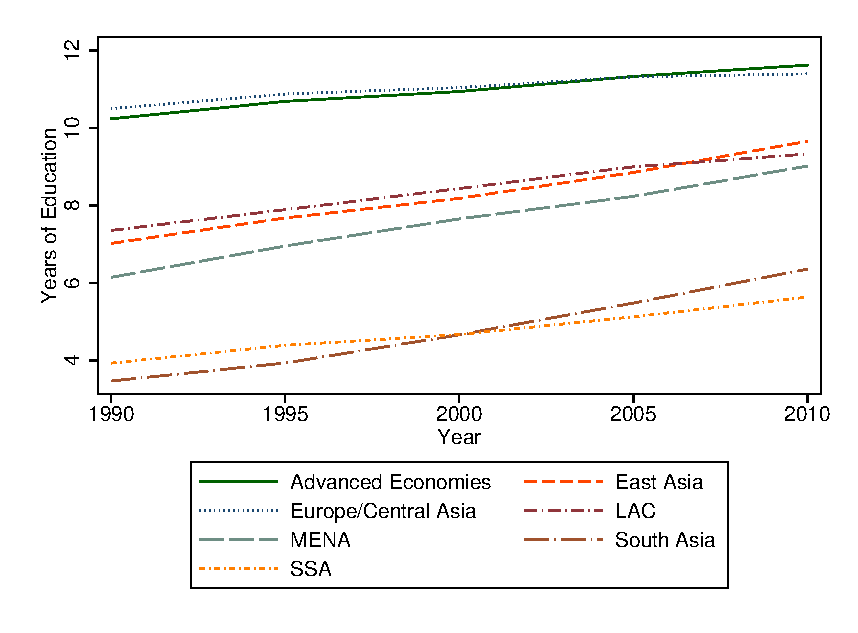
\includegraphics[scale=0.9]{\MMRfolder/Results/graphs/trends/SchoolingRegion.eps} 
\end{center}
\end{figure}

\begin{figure}[h!]
\begin{center}
\caption{Maternal Mortality Ratio by Region: 1990-2010}
\label{fig:MMRRegion}
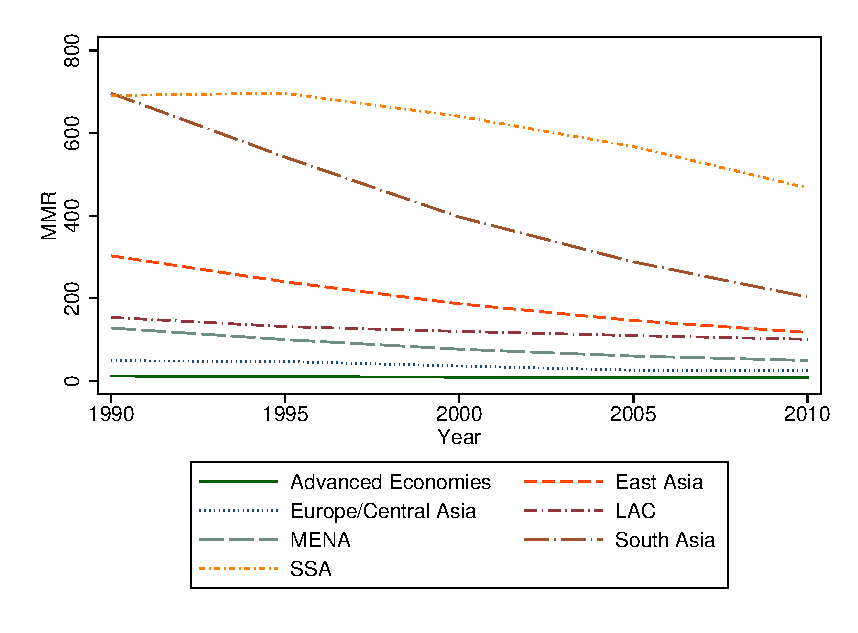
\includegraphics[scale=0.9]{\MMRfolder/Results/graphs/trends/MMRRegion.eps} 
\end{center}
\end{figure}

\begin{figure}[h!]
\begin{center}
\caption{Maternal Mortality and Education: Functional Form}
\label{fig:educmmr}
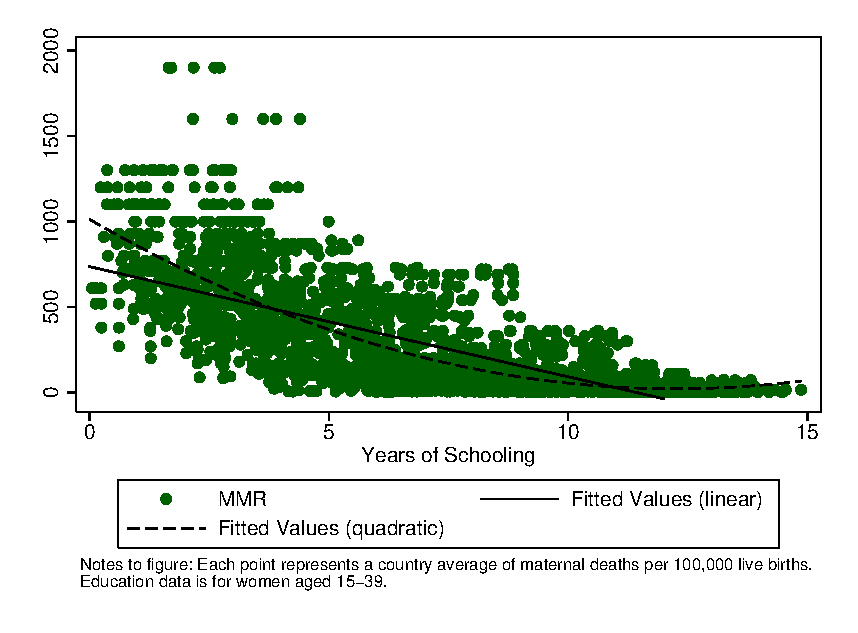
\includegraphics[scale=0.9]{\MMRfolder/Results/graphs/trends/Schooling_MMR_F.eps} 
\end{center}
\end{figure}

\begin{landscape}
\begin{figure}[h!]
\begin{center}
\caption{Maternal Mortality Ratio by Country}
\label{fig:MMRGlobal}
\includegraphics[scale=0.9]{\MMRfolder/Results_aug2013/Graphs/MMR_2010.eps} 
\end{center}
\end{figure}
\end{landscape}

\begin{figure}[htpb!]
  \begin{center}
    \caption{Maternal Mortality Ratio and Women's Education (Conditional on Income)}
    \label{MMRDeltaCond}
    \begin{subfigure}{.5\textwidth}
      \centering
      \includegraphics[scale=0.52]{\MMRfolder/Results/graphs/MMReducNDeltas_conditional.eps}
      \caption{Proportion out of School}
      \label{lowgdp}
    \end{subfigure}%
    \begin{subfigure}{.5\textwidth}
      \centering
      \includegraphics[scale=0.52]{\MMRfolder/Results/graphs/MMReducPDeltas_conditional.eps}
      \caption{Proportion in Primary School}
      \label{highgdp}
    \end{subfigure}
  \end{center}
  \floatfoot{\textsc{Notes to figure \ref{MMRDeltaCond}}: Each point
    represents the country average of $\Delta$ MMR and $\Delta$ educational indicator after
    conditioning on $\Delta$ GDP per capita.
    $\Delta$ is the first difference, and is a country average over the period 1990-2010
    (the full MMR sample).  The inverse of Proportion out of School is used, so $\Delta$
    is interpreted as a \emph{reduction} in the proportion of women out of school.
    Unconditional results are presented in figure 1 of the paper.}
\end{figure}

\begin{figure}[htpb!]
\begin{center}
\label{fig:margeffects}
\includegraphics[scale=0.88]{\MMRfolder/Results/graphs/marginsEducMMR.eps} 
\floatfoot{\textsc{Notes to figure \ref{fig:margeffects}}: Each point displays
  the estimated effect female of education on maternal mortality where education
  enters the regression equation as a quadratic term.  95\% confidence intervals
  are plotted along with estimated marginal effects.  Average years of schooling
  in the sample vary between 1.00 (Mozambique) to 12.91 (USA).}
\end{center}
\end{figure}



%\begin{figure}[htpb!]
%  \begin{center}
%    \caption{Marginal Effects of Female Education on Maternal Education (Quadratic)}
%    \label{fig:margeffects}
%    \begin{subfigure}{.5\textwidth}
%      \centering
%      \includegraphics[scale=0.52]{\MMRfolder/Results/graphs/marginsEducMMR.eps} 
%      \caption{Unconditional Estimates}
%      \label{margU}
%    \end{subfigure}%
%    \begin{subfigure}{.5\textwidth}
%      \centering
%      \includegraphics[scale=0.52]{\MMRfolder/Results/graphs/marginsEducMMR_FM.eps} 
%      \caption{Conditional on Male Education}
%      \label{margC}
%    \end{subfigure}
%  \end{center}
%\floatfoot{\textsc{Notes to figure \ref{fig:margeffects}}: Each point displays
%  the estimated effect female of education on maternal mortality where education
%  enters the regression equation as a quadratic term.  95\% confidence intervals
%  are plotted along with estimated marginal effects.  Average years of schooling
%  in the sample vary between 1.00 (Mozambique) to 12.91 (USA).}
%\end{figure}
